\documentclass{article}

\usepackage{amsmath}
\usepackage{amsfonts} % For math fonts.
\usepackage{amssymb} % For other math symbols not covered by amsmath.
\usepackage[pdftex]{graphicx} % For pictures, use \includegraphics[scale=decimal]{pic.png}; must be a .png file type.
\usepackage{multicol}
\usepackage{textcomp}
\usepackage[colorlinks = true, urlcolor = blue]{hyperref}
\usepackage{enumitem}
\usepackage{graphbox} 
\usepackage{subfig}
\usepackage{multicol}

\newcommand{\tab}{\hspace*{0.25in}}

\usepackage{tikz}
\usetikzlibrary{positioning, calc}
\usetikzlibrary{shapes.geometric,angles,quotes}


\usepackage{fullpage}
\usepackage{listings}
\lstset
{ %Formatting for code in appendix
    language=Python,
    basicstyle=\footnotesize,
    numbers=left,
    stepnumber=1,
    showstringspaces=false,
    tabsize=2,
    breaklines=true,
    breakatwhitespace=false,
}


\begin{document}


\begin{flushright}
Basics \& Basic I/O \end{flushright}

\vspace*{-1.5em}
\noindent\makebox[\linewidth]{\rule{\paperwidth}{0.4pt}}


\vspace*{2em}

\begin{enumerate}


%new_question
	\item Write a program that asks the user for \\
		\begin{minipage}{0.5\textwidth}	
		\vspace*{-0.5em}
			\begin{enumerate}  \setlength\itemsep{-0.3em}
				\item the year,
				\item the month, and
				\item the day	
			\end{enumerate} \vspace*{-1ex}
		and then outputs the date.
		\end{minipage}
		%\
		\begin{minipage}{0.5\textwidth}
			\centering
			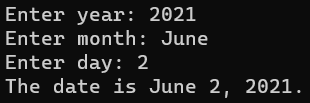
\includegraphics[scale=0.75]{./imgs/dateOutput.png}\\
			Your output should be similar to this.
		\end{minipage}

	


%new_question
	\item Write a program that asks the user for \\
		\begin{minipage}{0.5\textwidth}
		\vspace*{-0.5em}
			\begin{enumerate}  \setlength\itemsep{-0.3em}
				\item their first name and
				\item their age.  
			\end{enumerate} \vspace*{-1ex}
		and then outputs a greeting.
		\end{minipage}
		%\
		\begin{minipage}{0.5\textwidth}
			\centering
			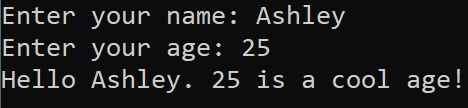
\includegraphics[scale=0.95]{./imgs/outputGreetingWithAge.png}\\
			Your output should be similar to this.
		\end{minipage}




%new_question
	\item 
		Write a program that asks the user for \\
		\begin{minipage}{0.5\textwidth}
		\vspace*{-0.5em}
			\begin{enumerate}  \setlength\itemsep{-0.3em}
				\item their first name and
				\item their last name.  
			\end{enumerate} \vspace*{-1ex}
		and then outputs a farewell.
		\end{minipage}
		%\
		\begin{minipage}{0.5\textwidth}
			\centering
			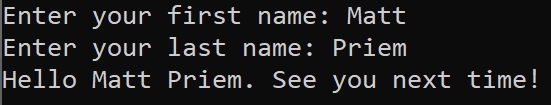
\includegraphics[scale=0.9]{./imgs/outputFarewell.png}\\
			Your output should be similar to this.
		\end{minipage}



%new_question
	\item 
		Write a program that asks the user for \\
		\begin{minipage}{0.5\textwidth}
		\vspace*{-0.5em}
			\begin{enumerate}  \setlength\itemsep{-0.3em}
				\item their first name and
				\item their last name.  
			\end{enumerate} \vspace*{-1ex}
		and then outputs a greeting.
		\end{minipage}
		%\
		\begin{minipage}{0.5\textwidth}
			\centering
			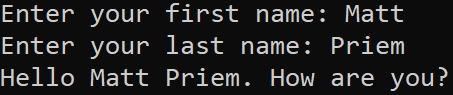
\includegraphics[scale=0.9]{./imgs/outputGreeting.png}\\
			Your output should be similar to this.
		\end{minipage}



%new_question
	\item 
		Write a program that asks the user for \\
		\begin{minipage}{0.5\textwidth}
		\vspace*{-0.5em}
			\begin{enumerate}  \setlength\itemsep{-0.3em}
				\item a color and
				\item an animal.  
			\end{enumerate} \vspace*{-1ex}
		and then outputs their pick.
		\end{minipage}
		%\
		\begin{minipage}{0.5\textwidth}
			\centering
			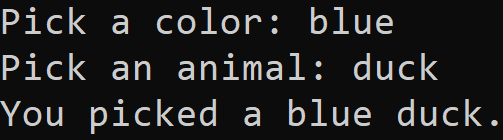
\includegraphics[scale=0.75]{./imgs/outputAnimalColor.png}\\
			Your output should be similar to this.
		\end{minipage}



%new_question
	\item 
		Write a program that asks the user for \\
		\begin{minipage}{0.5\textwidth}
		\vspace*{-0.5em}
			\begin{enumerate}  \setlength\itemsep{-0.3em}
				\item a food and
				\item a drink.  
			\end{enumerate} \vspace*{-1ex}
		and then outputs their order.
		\end{minipage}
		%\
		\begin{minipage}{0.5\textwidth}
			\centering
			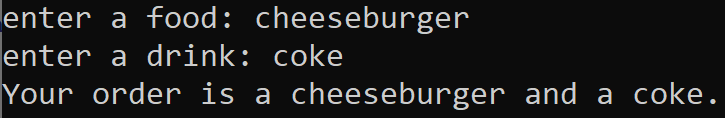
\includegraphics[scale=0.75]{./imgs/outputFoodAndDrink.png}\\
			Your output should be similar to this.
		\end{minipage}



%new_question
	\item 
		Write a program for an agreeable AI.\\
		The computer should ask the user for \\
		\begin{minipage}{0.5\textwidth}
		\vspace*{-0.5em}
			\begin{enumerate}  \setlength\itemsep{-0.3em}
				\item a color and
				\item a food.  
			\end{enumerate} \vspace*{-1ex}
		and then outputs their order.
		\end{minipage}
		%\
		\begin{minipage}{0.5\textwidth}
			\centering
			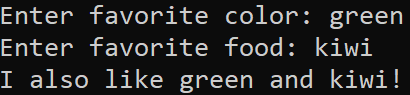
\includegraphics[scale=0.75]{./imgs/agreeableAIoutput.png}\\
			Your output should be similar to this.
		\end{minipage}


%new_question
	\item 
		Write a program that asks the user for \\
		\begin{minipage}{0.5\textwidth}
		\vspace*{-0.5em}
			\begin{enumerate}  \setlength\itemsep{-0.3em}
				\item a city and
				\item a state.  
			\end{enumerate} \vspace*{-1ex}
		and then outputs their order.
		\end{minipage}
		%\
		\begin{minipage}{0.5\textwidth}
			\centering
			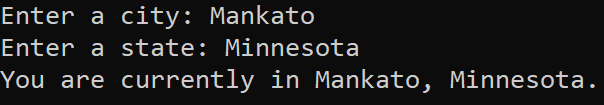
\includegraphics[scale=0.75]{./imgs/locationOutput.png}\\
			Your output should be similar to this.
		\end{minipage}


%new_question
	\item 
		Write code to swap the values of $x$ and $y$ using a temporary variable and without using
		the built-in function swap().\\		
		\begin{tabular}{|ll}
			\\			
			x = 3\\
			y = 7\\[5pt]
			\#Your code here. \\[5pt]
			& \\ & \\ & \\ & \\ & \\ & \\ & \\ & \\ & \\ & \\ 
		\end{tabular}






%end_of_questions



\end{enumerate}
\end{document}


